\documentclass[twoside]{book}

% Packages required by doxygen
\usepackage{fixltx2e}
\usepackage{calc}
\usepackage{doxygen}
\usepackage[export]{adjustbox} % also loads graphicx
\usepackage{graphicx}
\usepackage[utf8]{inputenc}
\usepackage{makeidx}
\usepackage{multicol}
\usepackage{multirow}
\PassOptionsToPackage{warn}{textcomp}
\usepackage{textcomp}
\usepackage[nointegrals]{wasysym}
\usepackage[table]{xcolor}

% Font selection
\usepackage[T1]{fontenc}
\usepackage[scaled=.90]{helvet}
\usepackage{courier}
\usepackage{amssymb}
\usepackage{sectsty}
\renewcommand{\familydefault}{\sfdefault}
\allsectionsfont{%
  \fontseries{bc}\selectfont%
  \color{darkgray}%
}
\renewcommand{\DoxyLabelFont}{%
  \fontseries{bc}\selectfont%
  \color{darkgray}%
}
\newcommand{\+}{\discretionary{\mbox{\scriptsize$\hookleftarrow$}}{}{}}

% Page & text layout
\usepackage{geometry}
\geometry{%
  a4paper,%
  top=2.5cm,%
  bottom=2.5cm,%
  left=2.5cm,%
  right=2.5cm%
}
\tolerance=750
\hfuzz=15pt
\hbadness=750
\setlength{\emergencystretch}{15pt}
\setlength{\parindent}{0cm}
\setlength{\parskip}{3ex plus 2ex minus 2ex}
\makeatletter
\renewcommand{\paragraph}{%
  \@startsection{paragraph}{4}{0ex}{-1.0ex}{1.0ex}{%
    \normalfont\normalsize\bfseries\SS@parafont%
  }%
}
\renewcommand{\subparagraph}{%
  \@startsection{subparagraph}{5}{0ex}{-1.0ex}{1.0ex}{%
    \normalfont\normalsize\bfseries\SS@subparafont%
  }%
}
\makeatother

% Headers & footers
\usepackage{fancyhdr}
\pagestyle{fancyplain}
\fancyhead[LE]{\fancyplain{}{\bfseries\thepage}}
\fancyhead[CE]{\fancyplain{}{}}
\fancyhead[RE]{\fancyplain{}{\bfseries\leftmark}}
\fancyhead[LO]{\fancyplain{}{\bfseries\rightmark}}
\fancyhead[CO]{\fancyplain{}{}}
\fancyhead[RO]{\fancyplain{}{\bfseries\thepage}}
\fancyfoot[LE]{\fancyplain{}{}}
\fancyfoot[CE]{\fancyplain{}{}}
\fancyfoot[RE]{\fancyplain{}{\bfseries\scriptsize Generated by Doxygen }}
\fancyfoot[LO]{\fancyplain{}{\bfseries\scriptsize Generated by Doxygen }}
\fancyfoot[CO]{\fancyplain{}{}}
\fancyfoot[RO]{\fancyplain{}{}}
\renewcommand{\footrulewidth}{0.4pt}
\renewcommand{\chaptermark}[1]{%
  \markboth{#1}{}%
}
\renewcommand{\sectionmark}[1]{%
  \markright{\thesection\ #1}%
}

% Indices & bibliography
\usepackage{natbib}
\usepackage[titles]{tocloft}
\setcounter{tocdepth}{3}
\setcounter{secnumdepth}{5}
\makeindex

% Hyperlinks (required, but should be loaded last)
\usepackage{ifpdf}
\ifpdf
  \usepackage[pdftex,pagebackref=true]{hyperref}
\else
  \usepackage[ps2pdf,pagebackref=true]{hyperref}
\fi
\hypersetup{%
  colorlinks=true,%
  linkcolor=blue,%
  citecolor=blue,%
  unicode%
}

% Custom commands
\newcommand{\clearemptydoublepage}{%
  \newpage{\pagestyle{empty}\cleardoublepage}%
}

\usepackage{caption}
\captionsetup{labelsep=space,justification=centering,font={bf},singlelinecheck=off,skip=4pt,position=top}

%===== C O N T E N T S =====

\begin{document}

% Titlepage & ToC
\hypersetup{pageanchor=false,
             bookmarksnumbered=true,
             pdfencoding=unicode
            }
\pagenumbering{alph}
\begin{titlepage}
\vspace*{7cm}
\begin{center}%
{\Large Heat\+Conduction }\\
\vspace*{1cm}
{\large Generated by Doxygen 1.8.13}\\
\end{center}
\end{titlepage}
\clearemptydoublepage
\pagenumbering{roman}
\tableofcontents
\clearemptydoublepage
\pagenumbering{arabic}
\hypersetup{pageanchor=true}

%--- Begin generated contents ---
\chapter{Hierarchical Index}
\section{Class Hierarchy}
This inheritance list is sorted roughly, but not completely, alphabetically\+:\begin{DoxyCompactList}
\item \contentsline{section}{Heat\+Conduction}{\pageref{class_heat_conduction}}{}
\begin{DoxyCompactList}
\item \contentsline{section}{Analytical\+Solution}{\pageref{class_analytical_solution}}{}
\item \contentsline{section}{Explicit\+Method}{\pageref{class_explicit_method}}{}
\begin{DoxyCompactList}
\item \contentsline{section}{Du\+Fort\+\_\+\+Frankel}{\pageref{class_du_fort___frankel}}{}
\item \contentsline{section}{Richardson}{\pageref{class_richardson}}{}
\end{DoxyCompactList}
\item \contentsline{section}{Implicit\+Method}{\pageref{class_implicit_method}}{}
\begin{DoxyCompactList}
\item \contentsline{section}{Crank\+Nicholson}{\pageref{class_crank_nicholson}}{}
\item \contentsline{section}{Laasonen}{\pageref{class_laasonen}}{}
\end{DoxyCompactList}
\end{DoxyCompactList}
\end{DoxyCompactList}

\chapter{Class Index}
\section{Class List}
Here are the classes, structs, unions and interfaces with brief descriptions\+:\begin{DoxyCompactList}
\item\contentsline{section}{\textbf{ Analytical\+Solution} \\*Sub Class used to calculate the analytical solution }{\pageref{class_analytical_solution}}{}
\item\contentsline{section}{\textbf{ Crank\+Nicholson} \\*Sub sub Class used to calculate the Crank-\/\+Nicholson scheme }{\pageref{class_crank_nicholson}}{}
\item\contentsline{section}{\textbf{ Du\+Fort\+\_\+\+Frankel} \\*Sub sub Class used to calculate the \doxyref{Du\+Fort\+\_\+\+Frankel}{p.}{class_du_fort___frankel} scheme }{\pageref{class_du_fort___frankel}}{}
\item\contentsline{section}{\textbf{ Explicit\+Method} \\*Sub Abstract Class used to calculate the Explicit scheme }{\pageref{class_explicit_method}}{}
\item\contentsline{section}{\textbf{ Heat\+Conduction} \\*Base abstract Class which include all the parameters to solve the problem }{\pageref{class_heat_conduction}}{}
\item\contentsline{section}{\textbf{ Implicit\+Method} \\*Sub Abstract Class used to calculate the Implicit scheme }{\pageref{class_implicit_method}}{}
\item\contentsline{section}{\textbf{ Laasonen} \\*Sub sub Class used to calculate the \doxyref{Laasonen}{p.}{class_laasonen} scheme }{\pageref{class_laasonen}}{}
\item\contentsline{section}{\textbf{ Richardson} \\*Sub sub Class used to calculate the \doxyref{Richardson}{p.}{class_richardson} scheme }{\pageref{class_richardson}}{}
\end{DoxyCompactList}

\chapter{File Index}
\section{File List}
Here is a list of all documented files with brief descriptions\+:\begin{DoxyCompactList}
\item\contentsline{section}{\textbf{ Heat\+Conduction.\+cpp} \\*Different objects to resolve an Heat Conduction problem }{\pageref{_heat_conduction_8cpp}}{}
\item\contentsline{section}{\textbf{ Heat\+Conduction.\+h} \\*Different objects to resolve an Heat Conduction problem }{\pageref{_heat_conduction_8h}}{}
\item\contentsline{section}{{\bfseries main.\+cpp} }{\pageref{main_8cpp}}{}
\item\contentsline{section}{\textbf{ Norms.\+cpp} \\*Functions to calculates norms }{\pageref{_norms_8cpp}}{}
\item\contentsline{section}{\textbf{ Norms.\+h} \\*Functions to calculates norms }{\pageref{_norms_8h}}{}
\end{DoxyCompactList}

\chapter{Class Documentation}
\hypertarget{class_analytical_solution}{}\section{Analytical\+Solution Class Reference}
\label{class_analytical_solution}\index{Analytical\+Solution@{Analytical\+Solution}}


Sub Class used to calculate the analytical solution.  




{\ttfamily \#include $<$Heat\+Conduction.\+h$>$}



Inheritance diagram for Analytical\+Solution\+:\nopagebreak
\begin{figure}[H]
\begin{center}
\leavevmode
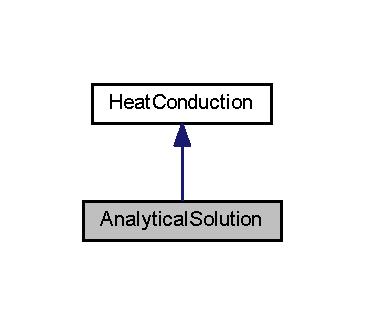
\includegraphics[width=175pt]{class_analytical_solution__inherit__graph}
\end{center}
\end{figure}


Collaboration diagram for Analytical\+Solution\+:\nopagebreak
\begin{figure}[H]
\begin{center}
\leavevmode
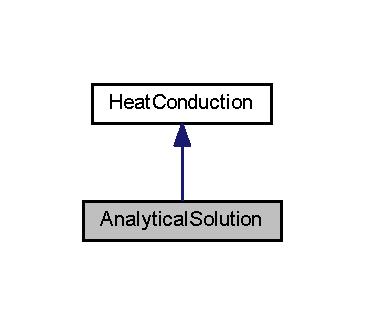
\includegraphics[width=175pt]{class_analytical_solution__coll__graph}
\end{center}
\end{figure}
\subsection*{Public Member Functions}
\begin{DoxyCompactItemize}
\item 
\hyperlink{class_analytical_solution_aaf001fd885d8a79df5609a484aac8430}{Analytical\+Solution} (double \hyperlink{class_heat_conduction_a2487010bf67582643ff59c0c5167725e}{Tin\+\_\+0}, double \hyperlink{class_heat_conduction_aeb50fb3189fd6545f765ef73c9be7889}{Text\+\_\+0}, double \hyperlink{class_heat_conduction_a6ccf374e13ab91b2403db617c9e7a8f0}{Xmin}, double \hyperlink{class_heat_conduction_a187dd05134300536dd9b5418e2957e9a}{Xmax}, double \hyperlink{class_heat_conduction_ab1d00caf79f4c04b420189eaf7c666e1}{Tend}, double \hyperlink{class_heat_conduction_a197d8aa3aa8619edaa640c243bdfc793}{D}, double \hyperlink{class_heat_conduction_a208bf1f475147b07a1f7d28533d78d9c}{dx}, double \hyperlink{class_heat_conduction_a7a7d5f6631039781c80b8c0c60e540e6}{dt})
\begin{DoxyCompactList}\small\item\em Constructor of the \hyperlink{class_analytical_solution}{Analytical\+Solution} class. \end{DoxyCompactList}\item 
virtual void \hyperlink{class_analytical_solution_afd1d8d955abbe0c5b7763544faad8dd2}{solve} ()
\begin{DoxyCompactList}\small\item\em Solve with the analytical solution. \end{DoxyCompactList}\end{DoxyCompactItemize}
\subsection*{Additional Inherited Members}


\subsection{Detailed Description}
Sub Class used to calculate the analytical solution. 

\hyperlink{class_analytical_solution}{Analytical\+Solution} is a sub class of \hyperlink{class_heat_conduction}{Heat\+Conduction}. It use the attribut of the mother class to calculate the analytical solution. 

Definition at line 56 of file Heat\+Conduction.\+h.



\subsection{Constructor \& Destructor Documentation}
\mbox{\Hypertarget{class_analytical_solution_aaf001fd885d8a79df5609a484aac8430}\label{class_analytical_solution_aaf001fd885d8a79df5609a484aac8430}} 
\index{Analytical\+Solution@{Analytical\+Solution}!Analytical\+Solution@{Analytical\+Solution}}
\index{Analytical\+Solution@{Analytical\+Solution}!Analytical\+Solution@{Analytical\+Solution}}
\subsubsection{\texorpdfstring{Analytical\+Solution()}{AnalyticalSolution()}}
{\footnotesize\ttfamily Analytical\+Solution\+::\+Analytical\+Solution (\begin{DoxyParamCaption}\item[{double}]{Tin\+\_\+0,  }\item[{double}]{Text\+\_\+0,  }\item[{double}]{Xmin,  }\item[{double}]{Xmax,  }\item[{double}]{Tend,  }\item[{double}]{D,  }\item[{double}]{dx,  }\item[{double}]{dt }\end{DoxyParamCaption})}



Constructor of the \hyperlink{class_analytical_solution}{Analytical\+Solution} class. 


\begin{DoxyParams}{Parameters}
{\em Tin\+\_\+0} & -\/ initial condition Temperature inside \\
\hline
{\em Text\+\_\+0} & -\/ initial condition Temperature outside \\
\hline
{\em Xmin} & -\/ the X position far left \\
\hline
{\em Xmax} & -\/ the X position far right \\
\hline
{\em Tend} & -\/ the end time of the simulation \\
\hline
{\em D} & -\/ the difusivity of the wall \\
\hline
{\em dx} & -\/ the space step \\
\hline
{\em dt} & -\/ the time step \\
\hline
\end{DoxyParams}


Definition at line 92 of file Heat\+Conduction.\+cpp.



\subsection{Member Function Documentation}
\mbox{\Hypertarget{class_analytical_solution_afd1d8d955abbe0c5b7763544faad8dd2}\label{class_analytical_solution_afd1d8d955abbe0c5b7763544faad8dd2}} 
\index{Analytical\+Solution@{Analytical\+Solution}!solve@{solve}}
\index{solve@{solve}!Analytical\+Solution@{Analytical\+Solution}}
\subsubsection{\texorpdfstring{solve()}{solve()}}
{\footnotesize\ttfamily void Analytical\+Solution\+::solve (\begin{DoxyParamCaption}{ }\end{DoxyParamCaption})\hspace{0.3cm}{\ttfamily [virtual]}}



Solve with the analytical solution. 

\begin{DoxyReturn}{Returns}
void -\/ the result is stored in the vector u\+\_\+n of the mother Class 
\end{DoxyReturn}


Reimplemented from \hyperlink{class_heat_conduction_ac176ea1a94c2fdb0da017b987ea22d1c}{Heat\+Conduction}.



Definition at line 100 of file Heat\+Conduction.\+cpp.



The documentation for this class was generated from the following files\+:\begin{DoxyCompactItemize}
\item 
\hyperlink{_heat_conduction_8h}{Heat\+Conduction.\+h}\item 
\hyperlink{_heat_conduction_8cpp}{Heat\+Conduction.\+cpp}\end{DoxyCompactItemize}

\hypertarget{class_crank_nicholson}{}\section{Crank\+Nicholson Class Reference}
\label{class_crank_nicholson}\index{Crank\+Nicholson@{Crank\+Nicholson}}


Sub sub Class used to calculate the Crank-\/\+Nicholson scheme.  




{\ttfamily \#include $<$Heat\+Conduction.\+h$>$}



Inheritance diagram for Crank\+Nicholson\+:
\nopagebreak
\begin{figure}[H]
\begin{center}
\leavevmode
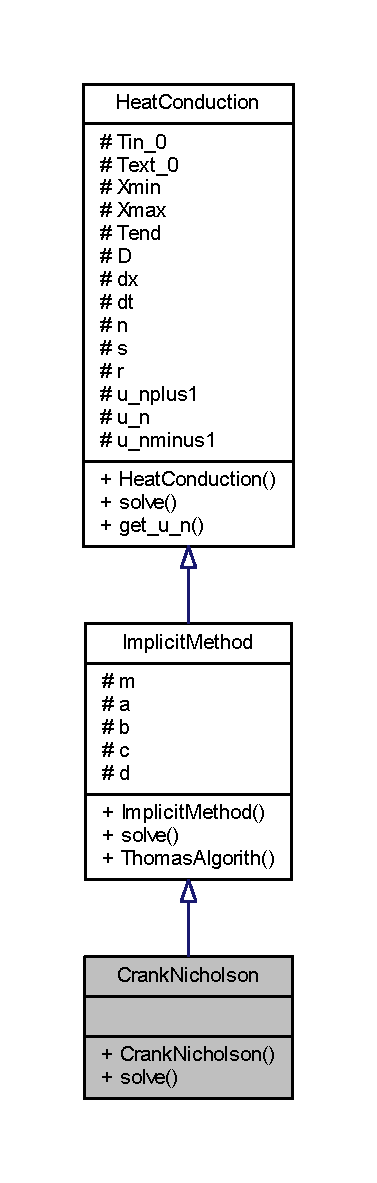
\includegraphics[height=550pt]{class_crank_nicholson__inherit__graph}
\end{center}
\end{figure}


Collaboration diagram for Crank\+Nicholson\+:
\nopagebreak
\begin{figure}[H]
\begin{center}
\leavevmode
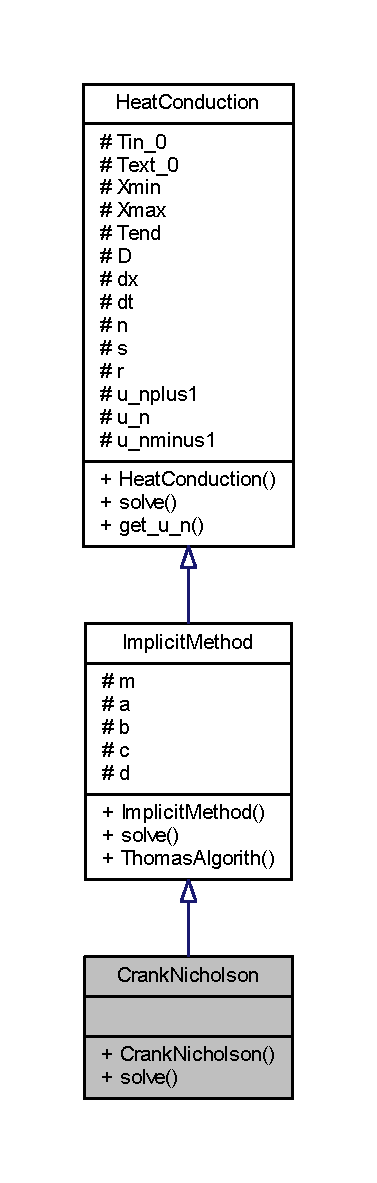
\includegraphics[height=550pt]{class_crank_nicholson__coll__graph}
\end{center}
\end{figure}
\subsection*{Public Member Functions}
\begin{DoxyCompactItemize}
\item 
\hyperlink{class_crank_nicholson_ac14a4b871ca88ddc37e85990f16a3904}{Crank\+Nicholson} (double \hyperlink{class_heat_conduction_a2487010bf67582643ff59c0c5167725e}{Tin\+\_\+0}, double \hyperlink{class_heat_conduction_aeb50fb3189fd6545f765ef73c9be7889}{Text\+\_\+0}, double \hyperlink{class_heat_conduction_a6ccf374e13ab91b2403db617c9e7a8f0}{Xmin}, double \hyperlink{class_heat_conduction_a187dd05134300536dd9b5418e2957e9a}{Xmax}, double \hyperlink{class_heat_conduction_ab1d00caf79f4c04b420189eaf7c666e1}{Tend}, double \hyperlink{class_heat_conduction_a197d8aa3aa8619edaa640c243bdfc793}{D}, double \hyperlink{class_heat_conduction_a208bf1f475147b07a1f7d28533d78d9c}{dx}, double \hyperlink{class_heat_conduction_a7a7d5f6631039781c80b8c0c60e540e6}{dt})
\begin{DoxyCompactList}\small\item\em Constructor of the \hyperlink{class_laasonen}{Laasonen} class. \end{DoxyCompactList}\item 
virtual void \hyperlink{class_crank_nicholson_a2846912cccce367888c37bf0e58f1cb1}{solve} ()
\begin{DoxyCompactList}\small\item\em Solve method. The matrix abc and the vector d are define after the Crank-\/\+Nicholson scheme. \end{DoxyCompactList}\end{DoxyCompactItemize}
\subsection*{Additional Inherited Members}


\subsection{Detailed Description}
Sub sub Class used to calculate the Crank-\/\+Nicholson scheme. 

\hyperlink{class_crank_nicholson}{Crank\+Nicholson} is a sub class of \hyperlink{class_implicit_method}{Implicit\+Method}. It use the Crank-\/\+Nicholson scheme, an implicit scheme to calculate an Heat Conduction problem of a wall which have a temperature imposed at the extremities. 

Definition at line 152 of file Heat\+Conduction.\+h.



\subsection{Constructor \& Destructor Documentation}
\mbox{\Hypertarget{class_crank_nicholson_ac14a4b871ca88ddc37e85990f16a3904}\label{class_crank_nicholson_ac14a4b871ca88ddc37e85990f16a3904}} 
\index{Crank\+Nicholson@{Crank\+Nicholson}!Crank\+Nicholson@{Crank\+Nicholson}}
\index{Crank\+Nicholson@{Crank\+Nicholson}!Crank\+Nicholson@{Crank\+Nicholson}}
\subsubsection{\texorpdfstring{Crank\+Nicholson()}{CrankNicholson()}}
{\footnotesize\ttfamily Crank\+Nicholson\+::\+Crank\+Nicholson (\begin{DoxyParamCaption}\item[{double}]{Tin\+\_\+0,  }\item[{double}]{Text\+\_\+0,  }\item[{double}]{Xmin,  }\item[{double}]{Xmax,  }\item[{double}]{Tend,  }\item[{double}]{D,  }\item[{double}]{dx,  }\item[{double}]{dt }\end{DoxyParamCaption})}



Constructor of the \hyperlink{class_laasonen}{Laasonen} class. 


\begin{DoxyParams}{Parameters}
{\em Tin\+\_\+0} & -\/ initial condition Temperature inside \\
\hline
{\em Text\+\_\+0} & -\/ initial condition Temperature outside \\
\hline
{\em Xmin} & -\/ the X position far left \\
\hline
{\em Xmax} & -\/ the X position far right \\
\hline
{\em Tend} & -\/ the end time of the simulation \\
\hline
{\em D} & -\/ the difusivity of the wall \\
\hline
{\em dx} & -\/ the space step \\
\hline
{\em dt} & -\/ the time step \\
\hline
\end{DoxyParams}


Definition at line 340 of file Heat\+Conduction.\+cpp.



\subsection{Member Function Documentation}
\mbox{\Hypertarget{class_crank_nicholson_a2846912cccce367888c37bf0e58f1cb1}\label{class_crank_nicholson_a2846912cccce367888c37bf0e58f1cb1}} 
\index{Crank\+Nicholson@{Crank\+Nicholson}!solve@{solve}}
\index{solve@{solve}!Crank\+Nicholson@{Crank\+Nicholson}}
\subsubsection{\texorpdfstring{solve()}{solve()}}
{\footnotesize\ttfamily void Crank\+Nicholson\+::solve (\begin{DoxyParamCaption}{ }\end{DoxyParamCaption})\hspace{0.3cm}{\ttfamily [virtual]}}



Solve method. The matrix abc and the vector d are define after the Crank-\/\+Nicholson scheme. 

\begin{DoxyReturn}{Returns}
void -\/ the result is stored in the vector u\+\_\+n of the mother Class 
\end{DoxyReturn}


Reimplemented from \hyperlink{class_implicit_method_ae06909ac3cde1ae9fb216501c852e22c}{Implicit\+Method}.



Definition at line 348 of file Heat\+Conduction.\+cpp.

Here is the call graph for this function\+:\nopagebreak
\begin{figure}[H]
\begin{center}
\leavevmode
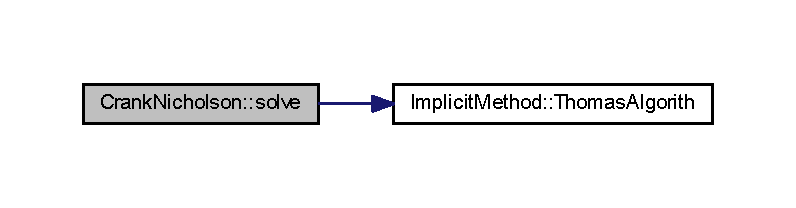
\includegraphics[width=350pt]{class_crank_nicholson_a2846912cccce367888c37bf0e58f1cb1_cgraph}
\end{center}
\end{figure}


The documentation for this class was generated from the following files\+:\begin{DoxyCompactItemize}
\item 
\hyperlink{_heat_conduction_8h}{Heat\+Conduction.\+h}\item 
\hyperlink{_heat_conduction_8cpp}{Heat\+Conduction.\+cpp}\end{DoxyCompactItemize}

\hypertarget{class_du_fort___frankel}{}\section{Du\+Fort\+\_\+\+Frankel Class Reference}
\label{class_du_fort___frankel}\index{Du\+Fort\+\_\+\+Frankel@{Du\+Fort\+\_\+\+Frankel}}


Sub sub Class used to calculate the \hyperlink{class_du_fort___frankel}{Du\+Fort\+\_\+\+Frankel} scheme.  




{\ttfamily \#include $<$Heat\+Conduction.\+h$>$}



Inheritance diagram for Du\+Fort\+\_\+\+Frankel\+:\nopagebreak
\begin{figure}[H]
\begin{center}
\leavevmode
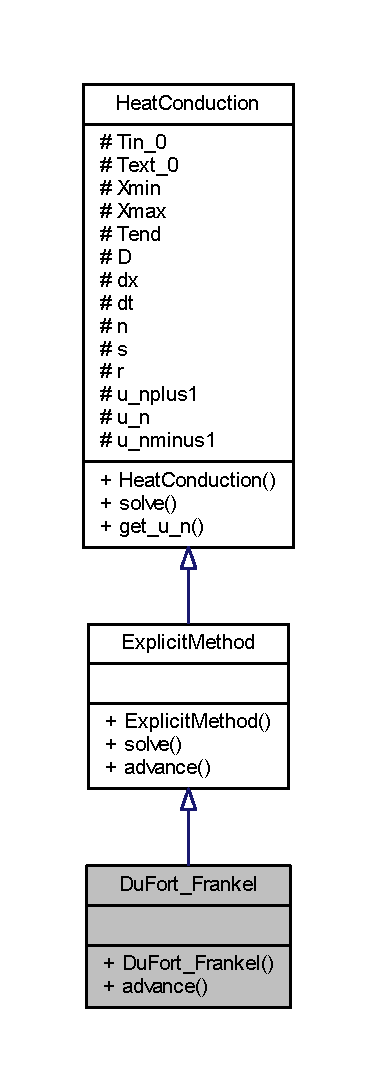
\includegraphics[width=166pt]{class_du_fort___frankel__inherit__graph}
\end{center}
\end{figure}


Collaboration diagram for Du\+Fort\+\_\+\+Frankel\+:\nopagebreak
\begin{figure}[H]
\begin{center}
\leavevmode
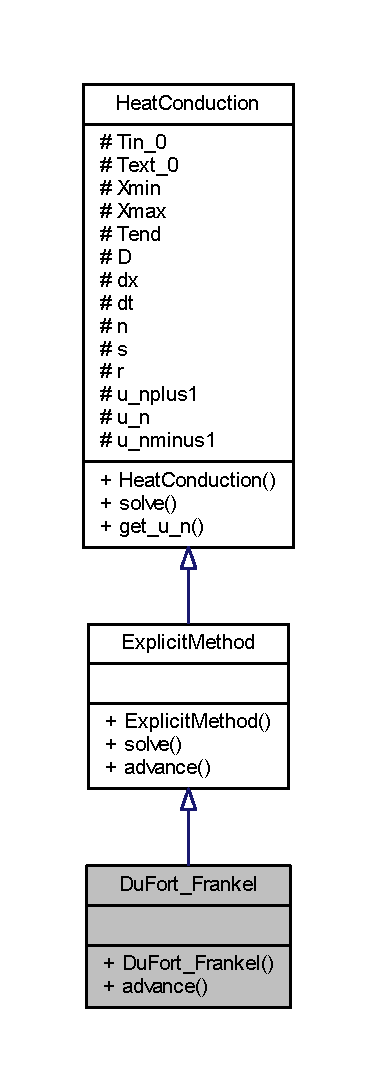
\includegraphics[width=166pt]{class_du_fort___frankel__coll__graph}
\end{center}
\end{figure}
\subsection*{Public Member Functions}
\begin{DoxyCompactItemize}
\item 
\hyperlink{class_du_fort___frankel_a5076e52da09f994da1542d71a56781df}{Du\+Fort\+\_\+\+Frankel} (double \hyperlink{class_heat_conduction_a2487010bf67582643ff59c0c5167725e}{Tin\+\_\+0}, double \hyperlink{class_heat_conduction_aeb50fb3189fd6545f765ef73c9be7889}{Text\+\_\+0}, double \hyperlink{class_heat_conduction_a6ccf374e13ab91b2403db617c9e7a8f0}{Xmin}, double \hyperlink{class_heat_conduction_a187dd05134300536dd9b5418e2957e9a}{Xmax}, double \hyperlink{class_heat_conduction_ab1d00caf79f4c04b420189eaf7c666e1}{Tend}, double \hyperlink{class_heat_conduction_a197d8aa3aa8619edaa640c243bdfc793}{D}, double \hyperlink{class_heat_conduction_a208bf1f475147b07a1f7d28533d78d9c}{dx}, double \hyperlink{class_heat_conduction_a7a7d5f6631039781c80b8c0c60e540e6}{dt})
\begin{DoxyCompactList}\small\item\em Constructor of the \hyperlink{class_du_fort___frankel}{Du\+Fort\+\_\+\+Frankel} class. \end{DoxyCompactList}\item 
virtual void \hyperlink{class_du_fort___frankel_ae8a6c6c56b2a4ce3bf7f80075a2cf680}{advance} (int i)
\begin{DoxyCompactList}\small\item\em Calcul of un\+\_\+plus1 according to \hyperlink{class_du_fort___frankel}{Du\+Fort\+\_\+\+Frankel} scheme. \end{DoxyCompactList}\end{DoxyCompactItemize}
\subsection*{Additional Inherited Members}


\subsection{Detailed Description}
Sub sub Class used to calculate the \hyperlink{class_du_fort___frankel}{Du\+Fort\+\_\+\+Frankel} scheme. 

\hyperlink{class_du_fort___frankel}{Du\+Fort\+\_\+\+Frankel} is a sub class of \hyperlink{class_explicit_method}{Explicit\+Method}. It use the Du\+Fort-\/\+Frankel scheme, a second order explicit scheme to calculate an Heat Conduction problem of a wall which have a temperature imposed at the extremities. 

Definition at line 107 of file Heat\+Conduction.\+h.



\subsection{Constructor \& Destructor Documentation}
\mbox{\Hypertarget{class_du_fort___frankel_a5076e52da09f994da1542d71a56781df}\label{class_du_fort___frankel_a5076e52da09f994da1542d71a56781df}} 
\index{Du\+Fort\+\_\+\+Frankel@{Du\+Fort\+\_\+\+Frankel}!Du\+Fort\+\_\+\+Frankel@{Du\+Fort\+\_\+\+Frankel}}
\index{Du\+Fort\+\_\+\+Frankel@{Du\+Fort\+\_\+\+Frankel}!Du\+Fort\+\_\+\+Frankel@{Du\+Fort\+\_\+\+Frankel}}
\subsubsection{\texorpdfstring{Du\+Fort\+\_\+\+Frankel()}{DuFort\_Frankel()}}
{\footnotesize\ttfamily Du\+Fort\+\_\+\+Frankel\+::\+Du\+Fort\+\_\+\+Frankel (\begin{DoxyParamCaption}\item[{double}]{Tin\+\_\+0,  }\item[{double}]{Text\+\_\+0,  }\item[{double}]{Xmin,  }\item[{double}]{Xmax,  }\item[{double}]{Tend,  }\item[{double}]{D,  }\item[{double}]{dx,  }\item[{double}]{dt }\end{DoxyParamCaption})}



Constructor of the \hyperlink{class_du_fort___frankel}{Du\+Fort\+\_\+\+Frankel} class. 


\begin{DoxyParams}{Parameters}
{\em Tin\+\_\+0} & -\/ initial condition Temperature inside \\
\hline
{\em Text\+\_\+0} & -\/ initial condition Temperature outside \\
\hline
{\em Xmin} & -\/ the X position far left \\
\hline
{\em Xmax} & -\/ the X position far right \\
\hline
{\em Tend} & -\/ the end time of the simulation \\
\hline
{\em D} & -\/ the difusivity of the wall \\
\hline
{\em dx} & -\/ the space step \\
\hline
{\em dt} & -\/ the time step \\
\hline
\end{DoxyParams}


Definition at line 242 of file Heat\+Conduction.\+cpp.



\subsection{Member Function Documentation}
\mbox{\Hypertarget{class_du_fort___frankel_ae8a6c6c56b2a4ce3bf7f80075a2cf680}\label{class_du_fort___frankel_ae8a6c6c56b2a4ce3bf7f80075a2cf680}} 
\index{Du\+Fort\+\_\+\+Frankel@{Du\+Fort\+\_\+\+Frankel}!advance@{advance}}
\index{advance@{advance}!Du\+Fort\+\_\+\+Frankel@{Du\+Fort\+\_\+\+Frankel}}
\subsubsection{\texorpdfstring{advance()}{advance()}}
{\footnotesize\ttfamily void Du\+Fort\+\_\+\+Frankel\+::advance (\begin{DoxyParamCaption}\item[{int}]{i }\end{DoxyParamCaption})\hspace{0.3cm}{\ttfamily [virtual]}}



Calcul of un\+\_\+plus1 according to \hyperlink{class_du_fort___frankel}{Du\+Fort\+\_\+\+Frankel} scheme. 


\begin{DoxyParams}{Parameters}
{\em i} & -\/ the space iteration at which is the solve method \\
\hline
\end{DoxyParams}
\begin{DoxyReturn}{Returns}
void -\/ the result is stored in the vector u\+\_\+nplus1 of the mother Class 
\end{DoxyReturn}


Reimplemented from \hyperlink{class_explicit_method_afdff9dbaacf767cdfe295103f3de41ef}{Explicit\+Method}.



Definition at line 251 of file Heat\+Conduction.\+cpp.



The documentation for this class was generated from the following files\+:\begin{DoxyCompactItemize}
\item 
\hyperlink{_heat_conduction_8h}{Heat\+Conduction.\+h}\item 
\hyperlink{_heat_conduction_8cpp}{Heat\+Conduction.\+cpp}\end{DoxyCompactItemize}

\hypertarget{class_explicit_method}{}\section{Explicit\+Method Class Reference}
\label{class_explicit_method}\index{Explicit\+Method@{Explicit\+Method}}


Sub Abstract Class used to calculate the Explicit scheme.  




{\ttfamily \#include $<$Heat\+Conduction.\+h$>$}



Inheritance diagram for Explicit\+Method\+:
\nopagebreak
\begin{figure}[H]
\begin{center}
\leavevmode
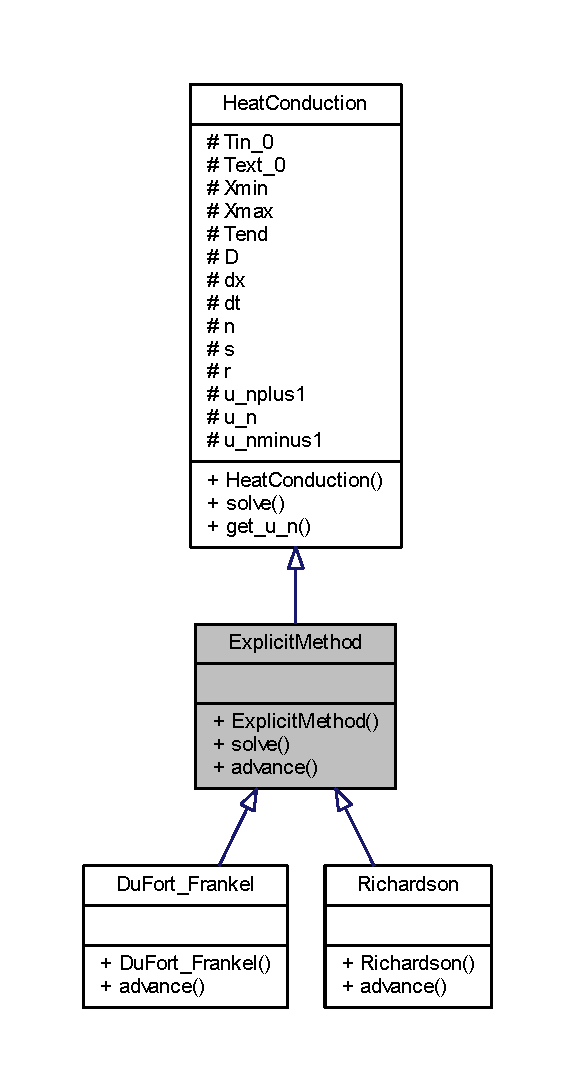
\includegraphics[width=276pt]{class_explicit_method__inherit__graph}
\end{center}
\end{figure}


Collaboration diagram for Explicit\+Method\+:
\nopagebreak
\begin{figure}[H]
\begin{center}
\leavevmode
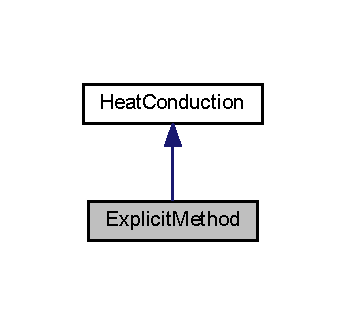
\includegraphics[width=181pt]{class_explicit_method__coll__graph}
\end{center}
\end{figure}
\subsection*{Public Member Functions}
\begin{DoxyCompactItemize}
\item 
\hyperlink{class_explicit_method_aa88329525eb6c640c7634792c933d3ea}{Explicit\+Method} (double \hyperlink{class_heat_conduction_a2487010bf67582643ff59c0c5167725e}{Tin\+\_\+0}, double \hyperlink{class_heat_conduction_aeb50fb3189fd6545f765ef73c9be7889}{Text\+\_\+0}, double \hyperlink{class_heat_conduction_a6ccf374e13ab91b2403db617c9e7a8f0}{Xmin}, double \hyperlink{class_heat_conduction_a187dd05134300536dd9b5418e2957e9a}{Xmax}, double \hyperlink{class_heat_conduction_ab1d00caf79f4c04b420189eaf7c666e1}{Tend}, double \hyperlink{class_heat_conduction_a197d8aa3aa8619edaa640c243bdfc793}{D}, double \hyperlink{class_heat_conduction_a208bf1f475147b07a1f7d28533d78d9c}{dx}, double \hyperlink{class_heat_conduction_a7a7d5f6631039781c80b8c0c60e540e6}{dt})
\begin{DoxyCompactList}\small\item\em Constructor of the \hyperlink{class_explicit_method}{Explicit\+Method} class. \end{DoxyCompactList}\item 
virtual void \hyperlink{class_explicit_method_a096efa29c4315794c60182e31c54a45e}{solve} ()
\begin{DoxyCompactList}\small\item\em Solve regroup the common part of the Explicit Method. \end{DoxyCompactList}\item 
virtual void \hyperlink{class_explicit_method_afdff9dbaacf767cdfe295103f3de41ef}{advance} (int i)
\begin{DoxyCompactList}\small\item\em Abstract method implemented in the sub sub classes. \end{DoxyCompactList}\end{DoxyCompactItemize}
\subsection*{Additional Inherited Members}


\subsection{Detailed Description}
Sub Abstract Class used to calculate the Explicit scheme. 

\hyperlink{class_explicit_method}{Explicit\+Method} is a sub class of \hyperlink{class_heat_conduction}{Heat\+Conduction}. Both explicit method share the same solve method, which is implemented in this class. The advance method is an abstract method implemented in the sub sub classes. 

Definition at line 70 of file Heat\+Conduction.\+h.



\subsection{Constructor \& Destructor Documentation}
\mbox{\Hypertarget{class_explicit_method_aa88329525eb6c640c7634792c933d3ea}\label{class_explicit_method_aa88329525eb6c640c7634792c933d3ea}} 
\index{Explicit\+Method@{Explicit\+Method}!Explicit\+Method@{Explicit\+Method}}
\index{Explicit\+Method@{Explicit\+Method}!Explicit\+Method@{Explicit\+Method}}
\subsubsection{\texorpdfstring{Explicit\+Method()}{ExplicitMethod()}}
{\footnotesize\ttfamily Explicit\+Method\+::\+Explicit\+Method (\begin{DoxyParamCaption}\item[{double}]{Tin\+\_\+0,  }\item[{double}]{Text\+\_\+0,  }\item[{double}]{Xmin,  }\item[{double}]{Xmax,  }\item[{double}]{Tend,  }\item[{double}]{D,  }\item[{double}]{dx,  }\item[{double}]{dt }\end{DoxyParamCaption})}



Constructor of the \hyperlink{class_explicit_method}{Explicit\+Method} class. 


\begin{DoxyParams}{Parameters}
{\em Tin\+\_\+0} & -\/ initial condition Temperature inside \\
\hline
{\em Text\+\_\+0} & -\/ initial condition Temperature outside \\
\hline
{\em Xmin} & -\/ the X position far left \\
\hline
{\em Xmax} & -\/ the X position far right \\
\hline
{\em Tend} & -\/ the end time of the simulation \\
\hline
{\em D} & -\/ the difusivity of the wall \\
\hline
{\em dx} & -\/ the space step \\
\hline
{\em dt} & -\/ the time step \\
\hline
\end{DoxyParams}


Definition at line 126 of file Heat\+Conduction.\+cpp.



\subsection{Member Function Documentation}
\mbox{\Hypertarget{class_explicit_method_afdff9dbaacf767cdfe295103f3de41ef}\label{class_explicit_method_afdff9dbaacf767cdfe295103f3de41ef}} 
\index{Explicit\+Method@{Explicit\+Method}!advance@{advance}}
\index{advance@{advance}!Explicit\+Method@{Explicit\+Method}}
\subsubsection{\texorpdfstring{advance()}{advance()}}
{\footnotesize\ttfamily void Explicit\+Method\+::advance (\begin{DoxyParamCaption}\item[{int}]{i }\end{DoxyParamCaption})\hspace{0.3cm}{\ttfamily [virtual]}}



Abstract method implemented in the sub sub classes. 


\begin{DoxyParams}{Parameters}
{\em i} & -\/ the space iteration at which is the solve method \\
\hline
\end{DoxyParams}
\begin{DoxyReturn}{Returns}
void -\/ the result is stored in the vector u\+\_\+nplus1 of the mother Class 
\end{DoxyReturn}


Reimplemented in \hyperlink{class_richardson_a9be0699e321b038d9361c209b3d542cb}{Richardson}, and \hyperlink{class_du_fort___frankel_ae8a6c6c56b2a4ce3bf7f80075a2cf680}{Du\+Fort\+\_\+\+Frankel}.



Definition at line 135 of file Heat\+Conduction.\+cpp.

Here is the caller graph for this function\+:\nopagebreak
\begin{figure}[H]
\begin{center}
\leavevmode
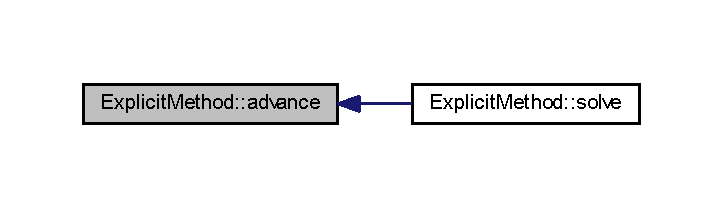
\includegraphics[width=347pt]{class_explicit_method_afdff9dbaacf767cdfe295103f3de41ef_icgraph}
\end{center}
\end{figure}
\mbox{\Hypertarget{class_explicit_method_a096efa29c4315794c60182e31c54a45e}\label{class_explicit_method_a096efa29c4315794c60182e31c54a45e}} 
\index{Explicit\+Method@{Explicit\+Method}!solve@{solve}}
\index{solve@{solve}!Explicit\+Method@{Explicit\+Method}}
\subsubsection{\texorpdfstring{solve()}{solve()}}
{\footnotesize\ttfamily void Explicit\+Method\+::solve (\begin{DoxyParamCaption}{ }\end{DoxyParamCaption})\hspace{0.3cm}{\ttfamily [virtual]}}



Solve regroup the common part of the Explicit Method. 

\begin{DoxyReturn}{Returns}
void -\/ the result is stored in the vector u\+\_\+n of the mother Class 
\end{DoxyReturn}


Reimplemented from \hyperlink{class_heat_conduction_ac176ea1a94c2fdb0da017b987ea22d1c}{Heat\+Conduction}.



Definition at line 143 of file Heat\+Conduction.\+cpp.

Here is the call graph for this function\+:\nopagebreak
\begin{figure}[H]
\begin{center}
\leavevmode
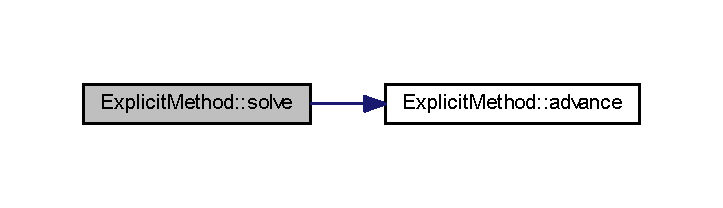
\includegraphics[width=347pt]{class_explicit_method_a096efa29c4315794c60182e31c54a45e_cgraph}
\end{center}
\end{figure}


The documentation for this class was generated from the following files\+:\begin{DoxyCompactItemize}
\item 
\hyperlink{_heat_conduction_8h}{Heat\+Conduction.\+h}\item 
\hyperlink{_heat_conduction_8cpp}{Heat\+Conduction.\+cpp}\end{DoxyCompactItemize}

\section{Heat\+Conduction Class Reference}
\label{class_heat_conduction}\index{Heat\+Conduction@{Heat\+Conduction}}


Base abstract Class which include all the parameters to solve the problem.  




{\ttfamily \#include $<$Heat\+Conduction.\+h$>$}

Inheritance diagram for Heat\+Conduction\+:\begin{figure}[H]
\begin{center}
\leavevmode
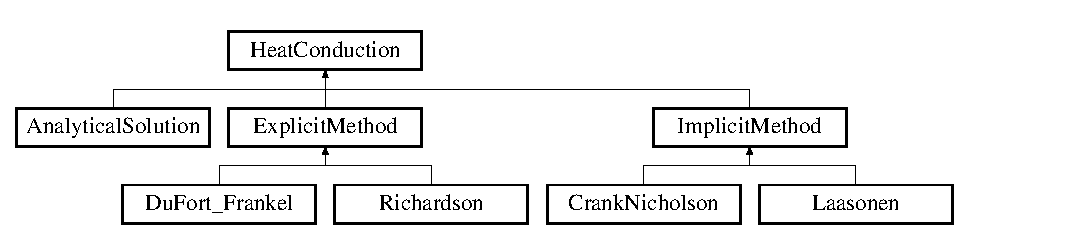
\includegraphics[height=2.776860cm]{class_heat_conduction}
\end{center}
\end{figure}
\subsection*{Public Member Functions}
\begin{DoxyCompactItemize}
\item 
\textbf{ Heat\+Conduction} (double \textbf{ Tin\+\_\+0}, double \textbf{ Text\+\_\+0}, double \textbf{ Xmin}, double \textbf{ Xmax}, double \textbf{ Tend}, double \textbf{ D}, double \textbf{ dx}, double \textbf{ dt})
\begin{DoxyCompactList}\small\item\em Constructor of the \doxyref{Heat\+Conduction}{p.}{class_heat_conduction} class. \end{DoxyCompactList}\item 
virtual void \textbf{ solve} ()
\begin{DoxyCompactList}\small\item\em Abstract solve. \end{DoxyCompactList}\item 
std\+::vector$<$ double $>$ \textbf{ get\+\_\+u\+\_\+n} () const
\begin{DoxyCompactList}\small\item\em Get method of the attribute u\+\_\+n. \end{DoxyCompactList}\end{DoxyCompactItemize}
\subsection*{Protected Attributes}
\begin{DoxyCompactItemize}
\item 
\mbox{\label{class_heat_conduction_a2487010bf67582643ff59c0c5167725e}} 
double \textbf{ Tin\+\_\+0}
\begin{DoxyCompactList}\small\item\em initial condition Temperature \end{DoxyCompactList}\item 
\mbox{\label{class_heat_conduction_aeb50fb3189fd6545f765ef73c9be7889}} 
double \textbf{ Text\+\_\+0}
\begin{DoxyCompactList}\small\item\em initial condition Temperature \end{DoxyCompactList}\item 
\mbox{\label{class_heat_conduction_a6ccf374e13ab91b2403db617c9e7a8f0}} 
double \textbf{ Xmin}
\begin{DoxyCompactList}\small\item\em initial condition Position \end{DoxyCompactList}\item 
\mbox{\label{class_heat_conduction_a187dd05134300536dd9b5418e2957e9a}} 
double \textbf{ Xmax}
\begin{DoxyCompactList}\small\item\em initial condition Position \end{DoxyCompactList}\item 
\mbox{\label{class_heat_conduction_ab1d00caf79f4c04b420189eaf7c666e1}} 
double \textbf{ Tend}
\begin{DoxyCompactList}\small\item\em initial condition Time \end{DoxyCompactList}\item 
\mbox{\label{class_heat_conduction_a197d8aa3aa8619edaa640c243bdfc793}} 
double \textbf{ D}
\begin{DoxyCompactList}\small\item\em initial condition D \end{DoxyCompactList}\item 
\mbox{\label{class_heat_conduction_a208bf1f475147b07a1f7d28533d78d9c}} 
double \textbf{ dx}
\begin{DoxyCompactList}\small\item\em space step \end{DoxyCompactList}\item 
\mbox{\label{class_heat_conduction_a7a7d5f6631039781c80b8c0c60e540e6}} 
double \textbf{ dt}
\begin{DoxyCompactList}\small\item\em time step \end{DoxyCompactList}\item 
\mbox{\label{class_heat_conduction_ada703cd81a60d17a134b15499bbbef98}} 
int \textbf{ n}
\begin{DoxyCompactList}\small\item\em number of time steps \end{DoxyCompactList}\item 
\mbox{\label{class_heat_conduction_ad380b438b1ab0f6988342ac4023854da}} 
int \textbf{ s}
\begin{DoxyCompactList}\small\item\em number of space steps \end{DoxyCompactList}\item 
\mbox{\label{class_heat_conduction_ae152528bd4b7d0841854b32d037ace72}} 
double \textbf{ r}
\begin{DoxyCompactList}\small\item\em calculation made once instead of multiple time \end{DoxyCompactList}\item 
\mbox{\label{class_heat_conduction_a6ad0488a3d4e3c9190b2abb3de8ccd2e}} 
std\+::vector$<$ double $>$ \textbf{ u\+\_\+nplus1}
\begin{DoxyCompactList}\small\item\em solution values vector n+1 \end{DoxyCompactList}\item 
\mbox{\label{class_heat_conduction_ac2e557e6d0c482dd49f78369c8d9f708}} 
std\+::vector$<$ double $>$ \textbf{ u\+\_\+n}
\begin{DoxyCompactList}\small\item\em solution values vector n \end{DoxyCompactList}\item 
\mbox{\label{class_heat_conduction_ae5bf8bf1144632fad72a415023ca4461}} 
std\+::vector$<$ double $>$ \textbf{ u\+\_\+nminus1}
\begin{DoxyCompactList}\small\item\em solution values vector n-\/1 \end{DoxyCompactList}\end{DoxyCompactItemize}


\subsection{Detailed Description}
Base abstract Class which include all the parameters to solve the problem. 

Heat Conduction is an object, in which attributes is a paramaters of the problem, and also have vectors which will be used to store the solution. It includes an abstract method solve, which will call the solve methods corresponding to the type of scheme the user need. 

Definition at line 27 of file Heat\+Conduction.\+h.



\subsection{Constructor \& Destructor Documentation}
\mbox{\label{class_heat_conduction_ab81631c27726b7048e49ac0b8fba9b23}} 
\index{Heat\+Conduction@{Heat\+Conduction}!Heat\+Conduction@{Heat\+Conduction}}
\index{Heat\+Conduction@{Heat\+Conduction}!Heat\+Conduction@{Heat\+Conduction}}
\subsubsection{Heat\+Conduction()}
{\footnotesize\ttfamily Heat\+Conduction\+::\+Heat\+Conduction (\begin{DoxyParamCaption}\item[{double}]{Tin\+\_\+0,  }\item[{double}]{Text\+\_\+0,  }\item[{double}]{Xmin,  }\item[{double}]{Xmax,  }\item[{double}]{Tend,  }\item[{double}]{D,  }\item[{double}]{dx,  }\item[{double}]{dt }\end{DoxyParamCaption})}



Constructor of the \doxyref{Heat\+Conduction}{p.}{class_heat_conduction} class. 


\begin{DoxyParams}{Parameters}
{\em Tin\+\_\+0} & -\/ initial condition Temperature inside \\
\hline
{\em Text\+\_\+0} & -\/ initial condition Temperature outside \\
\hline
{\em Xmin} & -\/ the X position far left \\
\hline
{\em Xmax} & -\/ the X position far right \\
\hline
{\em Tend} & -\/ the end time of the simulation \\
\hline
{\em D} & -\/ the difusivity of the wall \\
\hline
{\em dx} & -\/ the space step \\
\hline
{\em dt} & -\/ the time step \\
\hline
\end{DoxyParams}


Definition at line 38 of file Heat\+Conduction.\+cpp.



\subsection{Member Function Documentation}
\mbox{\label{class_heat_conduction_a97d3e5b07a0de19da5b1879208ae6bb3}} 
\index{Heat\+Conduction@{Heat\+Conduction}!get\+\_\+u\+\_\+n@{get\+\_\+u\+\_\+n}}
\index{get\+\_\+u\+\_\+n@{get\+\_\+u\+\_\+n}!Heat\+Conduction@{Heat\+Conduction}}
\subsubsection{get\+\_\+u\+\_\+n()}
{\footnotesize\ttfamily std\+::vector$<$ double $>$ Heat\+Conduction\+::get\+\_\+u\+\_\+n (\begin{DoxyParamCaption}{ }\end{DoxyParamCaption}) const}



Get method of the attribute u\+\_\+n. 


\begin{DoxyParams}{Parameters}
{\em none} & \\
\hline
\end{DoxyParams}
\begin{DoxyReturn}{Returns}
u\+\_\+n -\/ a vector attribute of the mother Class 
\end{DoxyReturn}


Definition at line 73 of file Heat\+Conduction.\+cpp.

\mbox{\label{class_heat_conduction_ac176ea1a94c2fdb0da017b987ea22d1c}} 
\index{Heat\+Conduction@{Heat\+Conduction}!solve@{solve}}
\index{solve@{solve}!Heat\+Conduction@{Heat\+Conduction}}
\subsubsection{solve()}
{\footnotesize\ttfamily void Heat\+Conduction\+::solve (\begin{DoxyParamCaption}{ }\end{DoxyParamCaption})\hspace{0.3cm}{\ttfamily [virtual]}}



Abstract solve. 


\begin{DoxyParams}{Parameters}
{\em none} & \\
\hline
\end{DoxyParams}
\begin{DoxyReturn}{Returns}
void -\/ the result is stored in the vector u\+\_\+n of the mother Class 
\end{DoxyReturn}


Reimplemented in \textbf{ Crank\+Nicholson} \doxyref{}{p.}{class_crank_nicholson_a2846912cccce367888c37bf0e58f1cb1}, \textbf{ Laasonen} \doxyref{}{p.}{class_laasonen_a53cf5a72691175df0b3b6bdcbfee8c9b}, \textbf{ Implicit\+Method} \doxyref{}{p.}{class_implicit_method_ae06909ac3cde1ae9fb216501c852e22c}, \textbf{ Explicit\+Method} \doxyref{}{p.}{class_explicit_method_a096efa29c4315794c60182e31c54a45e}, and \textbf{ Analytical\+Solution} \doxyref{}{p.}{class_analytical_solution_afd1d8d955abbe0c5b7763544faad8dd2}.



Definition at line 64 of file Heat\+Conduction.\+cpp.



The documentation for this class was generated from the following files\+:\begin{DoxyCompactItemize}
\item 
\textbf{ Heat\+Conduction.\+h}\item 
\textbf{ Heat\+Conduction.\+cpp}\end{DoxyCompactItemize}

\section{Implicit\+Method Class Reference}
\label{class_implicit_method}\index{Implicit\+Method@{Implicit\+Method}}


Sub Abstract Class used to calculate the Implicit scheme.  




{\ttfamily \#include $<$Heat\+Conduction.\+h$>$}

Inheritance diagram for Implicit\+Method\+:\begin{figure}[H]
\begin{center}
\leavevmode
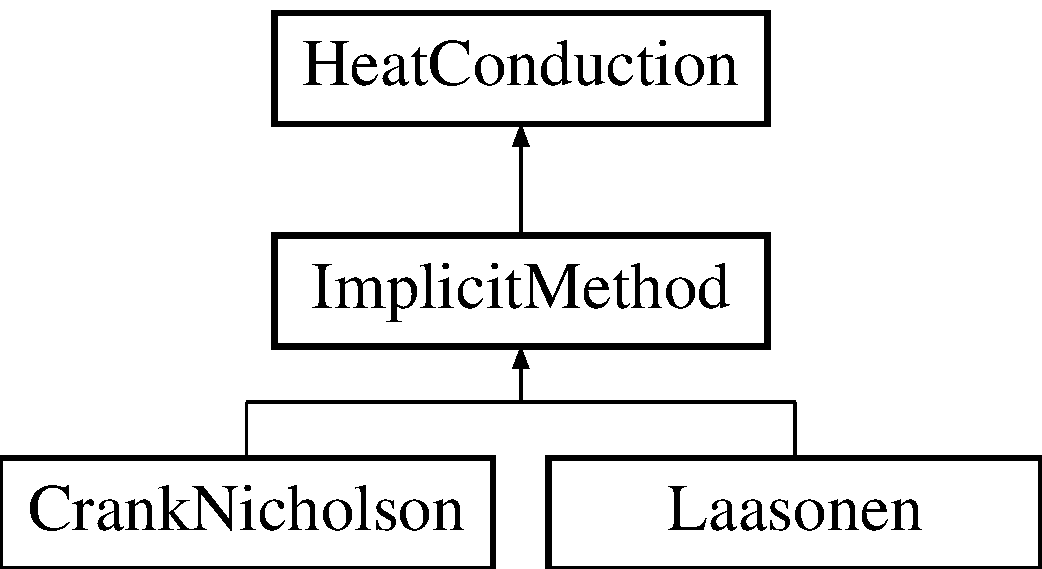
\includegraphics[height=3.000000cm]{class_implicit_method}
\end{center}
\end{figure}
\subsection*{Public Member Functions}
\begin{DoxyCompactItemize}
\item 
\textbf{ Implicit\+Method} (double \textbf{ Tin\+\_\+0}, double \textbf{ Text\+\_\+0}, double \textbf{ Xmin}, double \textbf{ Xmax}, double \textbf{ Tend}, double \textbf{ D}, double \textbf{ dx}, double \textbf{ dt})
\begin{DoxyCompactList}\small\item\em Constructor of the \doxyref{Implicit\+Method}{p.}{class_implicit_method} class. \end{DoxyCompactList}\item 
virtual void \textbf{ solve} ()
\begin{DoxyCompactList}\small\item\em Abstract solve. \end{DoxyCompactList}\item 
void \textbf{ Thomas\+Algorith} ()
\begin{DoxyCompactList}\small\item\em The Thomas Algorith, to solve Tridiagonal matrix problem. \end{DoxyCompactList}\end{DoxyCompactItemize}
\subsection*{Protected Attributes}
\begin{DoxyCompactItemize}
\item 
\mbox{\label{class_implicit_method_a40bd9e3fcd89952043c7c8a35011ba18}} 
double {\bfseries m}
\item 
\mbox{\label{class_implicit_method_a8fb476719886d49583938c8b40e4875e}} 
std\+::vector$<$ double $>$ {\bfseries a}
\item 
\mbox{\label{class_implicit_method_a2e2487e270f55de28c1f4db5d1b6bc0d}} 
std\+::vector$<$ double $>$ {\bfseries b}
\item 
\mbox{\label{class_implicit_method_aa66f38115300db94c12b7f95ad6c17f9}} 
std\+::vector$<$ double $>$ {\bfseries c}
\item 
\mbox{\label{class_implicit_method_a6e7d54136b7f6c21226b7de14b2308cb}} 
std\+::vector$<$ double $>$ {\bfseries d}
\end{DoxyCompactItemize}


\subsection{Detailed Description}
Sub Abstract Class used to calculate the Implicit scheme. 

\doxyref{Implicit\+Method}{p.}{class_implicit_method} is a sub class of \doxyref{Heat\+Conduction}{p.}{class_heat_conduction}. Both implicit method share the Thomas Algorith, which is implemented in this class. The solve method is an abstract method implemented in the sub sub classes. 

Definition at line 85 of file Heat\+Conduction.\+h.



\subsection{Constructor \& Destructor Documentation}
\mbox{\label{class_implicit_method_aa1169b777d7e6406f2a754da0fa9b515}} 
\index{Implicit\+Method@{Implicit\+Method}!Implicit\+Method@{Implicit\+Method}}
\index{Implicit\+Method@{Implicit\+Method}!Implicit\+Method@{Implicit\+Method}}
\subsubsection{Implicit\+Method()}
{\footnotesize\ttfamily Implicit\+Method\+::\+Implicit\+Method (\begin{DoxyParamCaption}\item[{double}]{Tin\+\_\+0,  }\item[{double}]{Text\+\_\+0,  }\item[{double}]{Xmin,  }\item[{double}]{Xmax,  }\item[{double}]{Tend,  }\item[{double}]{D,  }\item[{double}]{dx,  }\item[{double}]{dt }\end{DoxyParamCaption})}



Constructor of the \doxyref{Implicit\+Method}{p.}{class_implicit_method} class. 


\begin{DoxyParams}{Parameters}
{\em Tin\+\_\+0} & -\/ initial condition Temperature inside \\
\hline
{\em Text\+\_\+0} & -\/ initial condition Temperature outside \\
\hline
{\em Xmin} & -\/ the X position far left \\
\hline
{\em Xmax} & -\/ the X position far right \\
\hline
{\em Tend} & -\/ the end time of the simulation \\
\hline
{\em D} & -\/ the difusivity of the wall \\
\hline
{\em dx} & -\/ the space step \\
\hline
{\em dt} & -\/ the time step \\
\hline
\end{DoxyParams}


Definition at line 181 of file Heat\+Conduction.\+cpp.



\subsection{Member Function Documentation}
\mbox{\label{class_implicit_method_ae06909ac3cde1ae9fb216501c852e22c}} 
\index{Implicit\+Method@{Implicit\+Method}!solve@{solve}}
\index{solve@{solve}!Implicit\+Method@{Implicit\+Method}}
\subsubsection{solve()}
{\footnotesize\ttfamily void Implicit\+Method\+::solve (\begin{DoxyParamCaption}{ }\end{DoxyParamCaption})\hspace{0.3cm}{\ttfamily [virtual]}}



Abstract solve. 


\begin{DoxyParams}{Parameters}
{\em none} & \\
\hline
\end{DoxyParams}
\begin{DoxyReturn}{Returns}
void -\/ the result is stored in the vector u\+\_\+n of the mother Class 
\end{DoxyReturn}


Reimplemented from \textbf{ Heat\+Conduction} \doxyref{}{p.}{class_heat_conduction_ac176ea1a94c2fdb0da017b987ea22d1c}.



Reimplemented in \textbf{ Crank\+Nicholson} \doxyref{}{p.}{class_crank_nicholson_a2846912cccce367888c37bf0e58f1cb1}, and \textbf{ Laasonen} \doxyref{}{p.}{class_laasonen_a53cf5a72691175df0b3b6bdcbfee8c9b}.



Definition at line 203 of file Heat\+Conduction.\+cpp.

\mbox{\label{class_implicit_method_ae06f9aa9d076738cdcb7cd967d453795}} 
\index{Implicit\+Method@{Implicit\+Method}!Thomas\+Algorith@{Thomas\+Algorith}}
\index{Thomas\+Algorith@{Thomas\+Algorith}!Implicit\+Method@{Implicit\+Method}}
\subsubsection{Thomas\+Algorith()}
{\footnotesize\ttfamily void Implicit\+Method\+::\+Thomas\+Algorith (\begin{DoxyParamCaption}{ }\end{DoxyParamCaption})}



The Thomas Algorith, to solve Tridiagonal matrix problem. 


\begin{DoxyParams}{Parameters}
{\em none} & \\
\hline
\end{DoxyParams}
\begin{DoxyReturn}{Returns}
void -\/ the result is stored in the vector u\+\_\+n of the mother Class 
\end{DoxyReturn}


Definition at line 212 of file Heat\+Conduction.\+cpp.



The documentation for this class was generated from the following files\+:\begin{DoxyCompactItemize}
\item 
\textbf{ Heat\+Conduction.\+h}\item 
\textbf{ Heat\+Conduction.\+cpp}\end{DoxyCompactItemize}

\section{Laasonen Class Reference}
\label{class_laasonen}\index{Laasonen@{Laasonen}}


Sub sub Class used to calculate the \doxyref{Laasonen}{p.}{class_laasonen} scheme.  




{\ttfamily \#include $<$Heat\+Conduction.\+h$>$}

Inheritance diagram for Laasonen\+:\begin{figure}[H]
\begin{center}
\leavevmode
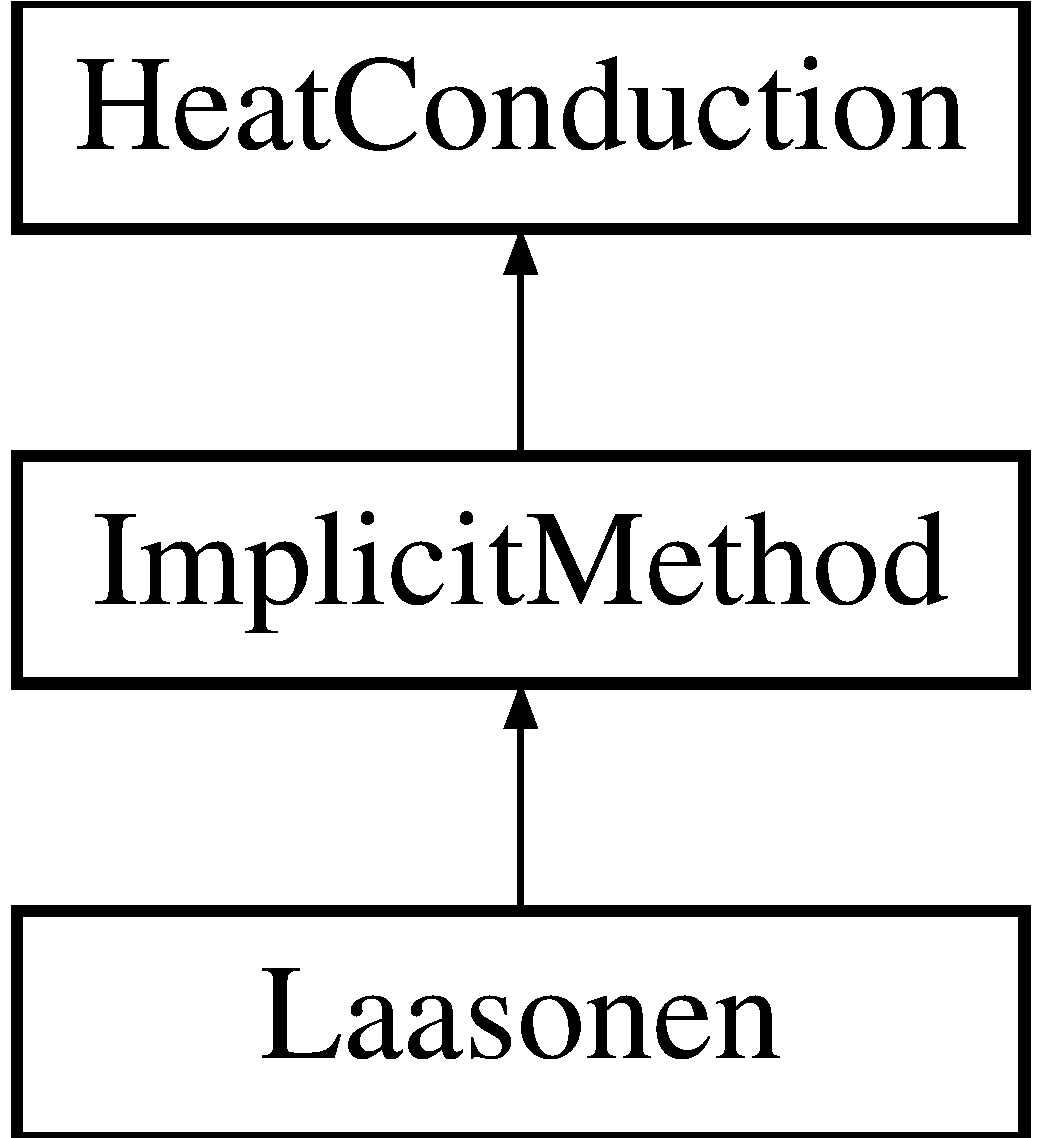
\includegraphics[height=3.000000cm]{class_laasonen}
\end{center}
\end{figure}
\subsection*{Public Member Functions}
\begin{DoxyCompactItemize}
\item 
\textbf{ Laasonen} (double \textbf{ Tin\+\_\+0}, double \textbf{ Text\+\_\+0}, double \textbf{ Xmin}, double \textbf{ Xmax}, double \textbf{ Tend}, double \textbf{ D}, double \textbf{ dx}, double \textbf{ dt})
\begin{DoxyCompactList}\small\item\em Constructor of the \doxyref{Laasonen}{p.}{class_laasonen} class. \end{DoxyCompactList}\item 
virtual void \textbf{ solve} ()
\begin{DoxyCompactList}\small\item\em Solve method. The matrix abc and the vector d are define after the \doxyref{Laasonen}{p.}{class_laasonen} scheme. \end{DoxyCompactList}\end{DoxyCompactItemize}
\subsection*{Additional Inherited Members}


\subsection{Detailed Description}
Sub sub Class used to calculate the \doxyref{Laasonen}{p.}{class_laasonen} scheme. 

\doxyref{Laasonen}{p.}{class_laasonen} is a sub class of \doxyref{Implicit\+Method}{p.}{class_implicit_method}. It use the \doxyref{Laasonen}{p.}{class_laasonen} scheme, an implicit scheme to calculate an Heat Conduction problem of a wall which have a temperature imposed at the extremities. 

Definition at line 137 of file Heat\+Conduction.\+h.



\subsection{Constructor \& Destructor Documentation}
\mbox{\label{class_laasonen_a31c8458bc908b985f992560b995b8d56}} 
\index{Laasonen@{Laasonen}!Laasonen@{Laasonen}}
\index{Laasonen@{Laasonen}!Laasonen@{Laasonen}}
\subsubsection{Laasonen()}
{\footnotesize\ttfamily Laasonen\+::\+Laasonen (\begin{DoxyParamCaption}\item[{double}]{Tin\+\_\+0,  }\item[{double}]{Text\+\_\+0,  }\item[{double}]{Xmin,  }\item[{double}]{Xmax,  }\item[{double}]{Tend,  }\item[{double}]{D,  }\item[{double}]{dx,  }\item[{double}]{dt }\end{DoxyParamCaption})}



Constructor of the \doxyref{Laasonen}{p.}{class_laasonen} class. 


\begin{DoxyParams}{Parameters}
{\em Tin\+\_\+0} & -\/ initial condition Temperature inside \\
\hline
{\em Text\+\_\+0} & -\/ initial condition Temperature outside \\
\hline
{\em Xmin} & -\/ the X position far left \\
\hline
{\em Xmax} & -\/ the X position far right \\
\hline
{\em Tend} & -\/ the end time of the simulation \\
\hline
{\em D} & -\/ the difusivity of the wall \\
\hline
{\em dx} & -\/ the space step \\
\hline
{\em dt} & -\/ the time step \\
\hline
\end{DoxyParams}


Definition at line 300 of file Heat\+Conduction.\+cpp.



\subsection{Member Function Documentation}
\mbox{\label{class_laasonen_a53cf5a72691175df0b3b6bdcbfee8c9b}} 
\index{Laasonen@{Laasonen}!solve@{solve}}
\index{solve@{solve}!Laasonen@{Laasonen}}
\subsubsection{solve()}
{\footnotesize\ttfamily void Laasonen\+::solve (\begin{DoxyParamCaption}{ }\end{DoxyParamCaption})\hspace{0.3cm}{\ttfamily [virtual]}}



Solve method. The matrix abc and the vector d are define after the \doxyref{Laasonen}{p.}{class_laasonen} scheme. 


\begin{DoxyParams}{Parameters}
{\em none} & \\
\hline
\end{DoxyParams}
\begin{DoxyReturn}{Returns}
void -\/ the result is stored in the vector u\+\_\+n of the mother Class 
\end{DoxyReturn}


Reimplemented from \textbf{ Implicit\+Method} \doxyref{}{p.}{class_implicit_method_ae06909ac3cde1ae9fb216501c852e22c}.



Definition at line 309 of file Heat\+Conduction.\+cpp.



The documentation for this class was generated from the following files\+:\begin{DoxyCompactItemize}
\item 
\textbf{ Heat\+Conduction.\+h}\item 
\textbf{ Heat\+Conduction.\+cpp}\end{DoxyCompactItemize}

\hypertarget{class_richardson}{}\section{Richardson Class Reference}
\label{class_richardson}\index{Richardson@{Richardson}}


Sub sub Class used to calculate the \hyperlink{class_richardson}{Richardson} scheme.  




{\ttfamily \#include $<$Heat\+Conduction.\+h$>$}



Inheritance diagram for Richardson\+:
\nopagebreak
\begin{figure}[H]
\begin{center}
\leavevmode
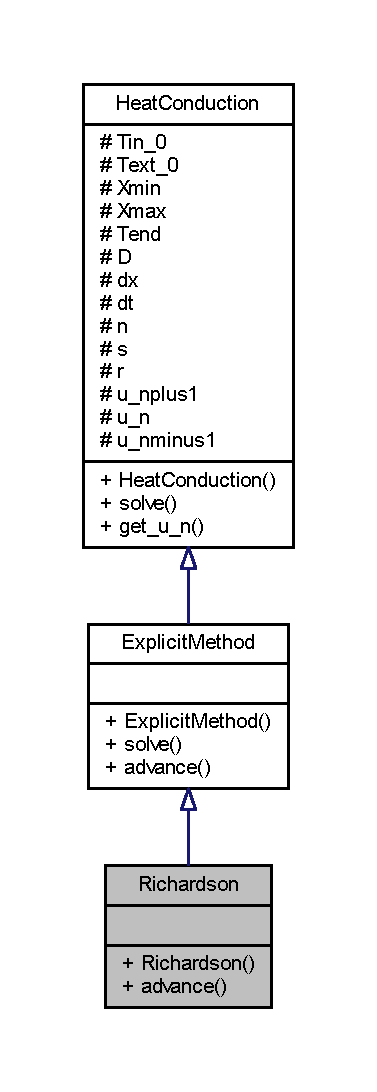
\includegraphics[width=181pt]{class_richardson__inherit__graph}
\end{center}
\end{figure}


Collaboration diagram for Richardson\+:
\nopagebreak
\begin{figure}[H]
\begin{center}
\leavevmode
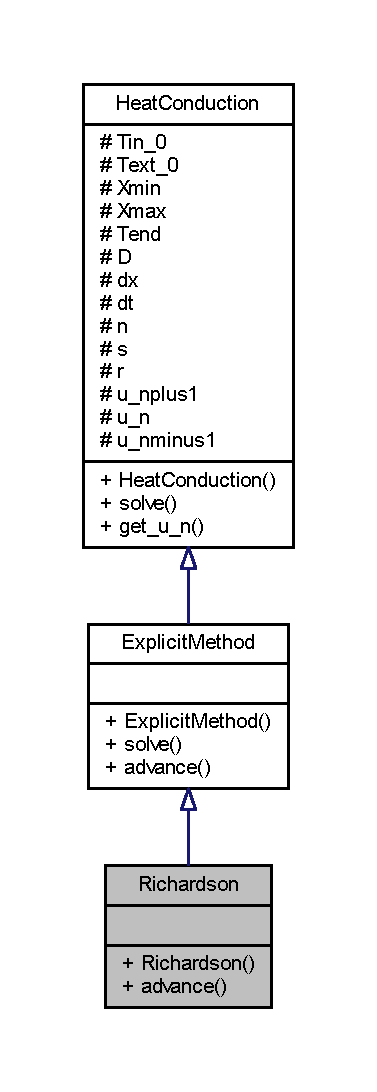
\includegraphics[width=181pt]{class_richardson__coll__graph}
\end{center}
\end{figure}
\subsection*{Public Member Functions}
\begin{DoxyCompactItemize}
\item 
\hyperlink{class_richardson_ae38842e27368e061f4f9ce3e692bcdbf}{Richardson} (double \hyperlink{class_heat_conduction_a2487010bf67582643ff59c0c5167725e}{Tin\+\_\+0}, double \hyperlink{class_heat_conduction_aeb50fb3189fd6545f765ef73c9be7889}{Text\+\_\+0}, double \hyperlink{class_heat_conduction_a6ccf374e13ab91b2403db617c9e7a8f0}{Xmin}, double \hyperlink{class_heat_conduction_a187dd05134300536dd9b5418e2957e9a}{Xmax}, double \hyperlink{class_heat_conduction_ab1d00caf79f4c04b420189eaf7c666e1}{Tend}, double \hyperlink{class_heat_conduction_a197d8aa3aa8619edaa640c243bdfc793}{D}, double \hyperlink{class_heat_conduction_a208bf1f475147b07a1f7d28533d78d9c}{dx}, double \hyperlink{class_heat_conduction_a7a7d5f6631039781c80b8c0c60e540e6}{dt})
\begin{DoxyCompactList}\small\item\em Constructor of the \hyperlink{class_richardson}{Richardson} class. \end{DoxyCompactList}\item 
virtual void \hyperlink{class_richardson_a9be0699e321b038d9361c209b3d542cb}{advance} (int i)
\begin{DoxyCompactList}\small\item\em Calcul of un\+\_\+plus1 according to \hyperlink{class_richardson}{Richardson} scheme. \end{DoxyCompactList}\end{DoxyCompactItemize}
\subsection*{Additional Inherited Members}


\subsection{Detailed Description}
Sub sub Class used to calculate the \hyperlink{class_richardson}{Richardson} scheme. 

\hyperlink{class_richardson}{Richardson} is a sub class of \hyperlink{class_explicit_method}{Explicit\+Method}. It use the \hyperlink{class_richardson}{Richardson} scheme, a second order explicit scheme to calculate an Heat Conduction problem of a wall which have a temperature imposed at the extremities. 

Definition at line 122 of file Heat\+Conduction.\+h.



\subsection{Constructor \& Destructor Documentation}
\mbox{\Hypertarget{class_richardson_ae38842e27368e061f4f9ce3e692bcdbf}\label{class_richardson_ae38842e27368e061f4f9ce3e692bcdbf}} 
\index{Richardson@{Richardson}!Richardson@{Richardson}}
\index{Richardson@{Richardson}!Richardson@{Richardson}}
\subsubsection{\texorpdfstring{Richardson()}{Richardson()}}
{\footnotesize\ttfamily Richardson\+::\+Richardson (\begin{DoxyParamCaption}\item[{double}]{Tin\+\_\+0,  }\item[{double}]{Text\+\_\+0,  }\item[{double}]{Xmin,  }\item[{double}]{Xmax,  }\item[{double}]{Tend,  }\item[{double}]{D,  }\item[{double}]{dx,  }\item[{double}]{dt }\end{DoxyParamCaption})}



Constructor of the \hyperlink{class_richardson}{Richardson} class. 


\begin{DoxyParams}{Parameters}
{\em Tin\+\_\+0} & -\/ initial condition Temperature inside \\
\hline
{\em Text\+\_\+0} & -\/ initial condition Temperature outside \\
\hline
{\em Xmin} & -\/ the X position far left \\
\hline
{\em Xmax} & -\/ the X position far right \\
\hline
{\em Tend} & -\/ the end time of the simulation \\
\hline
{\em D} & -\/ the difusivity of the wall \\
\hline
{\em dx} & -\/ the space step \\
\hline
{\em dt} & -\/ the time step \\
\hline
\end{DoxyParams}


Definition at line 268 of file Heat\+Conduction.\+cpp.



\subsection{Member Function Documentation}
\mbox{\Hypertarget{class_richardson_a9be0699e321b038d9361c209b3d542cb}\label{class_richardson_a9be0699e321b038d9361c209b3d542cb}} 
\index{Richardson@{Richardson}!advance@{advance}}
\index{advance@{advance}!Richardson@{Richardson}}
\subsubsection{\texorpdfstring{advance()}{advance()}}
{\footnotesize\ttfamily void Richardson\+::advance (\begin{DoxyParamCaption}\item[{int}]{i }\end{DoxyParamCaption})\hspace{0.3cm}{\ttfamily [virtual]}}



Calcul of un\+\_\+plus1 according to \hyperlink{class_richardson}{Richardson} scheme. 


\begin{DoxyParams}{Parameters}
{\em i} & -\/ the space iteration at which is the solve method \\
\hline
\end{DoxyParams}
\begin{DoxyReturn}{Returns}
void -\/ the result is stored in the vector u\+\_\+nplus1 of the mother Class 
\end{DoxyReturn}


Reimplemented from \hyperlink{class_explicit_method_afdff9dbaacf767cdfe295103f3de41ef}{Explicit\+Method}.



Definition at line 277 of file Heat\+Conduction.\+cpp.



The documentation for this class was generated from the following files\+:\begin{DoxyCompactItemize}
\item 
\hyperlink{_heat_conduction_8h}{Heat\+Conduction.\+h}\item 
\hyperlink{_heat_conduction_8cpp}{Heat\+Conduction.\+cpp}\end{DoxyCompactItemize}

\chapter{File Documentation}
\hypertarget{_heat_conduction_8cpp}{}\section{Heat\+Conduction.\+cpp File Reference}
\label{_heat_conduction_8cpp}\index{Heat\+Conduction.\+cpp@{Heat\+Conduction.\+cpp}}


Different objects to resolve an Heat Conduction problem.  


{\ttfamily \#include \char`\"{}Heat\+Conduction.\+h\char`\"{}}\newline
{\ttfamily \#include $<$cmath$>$}\newline
Include dependency graph for Heat\+Conduction.\+cpp\+:\nopagebreak
\begin{figure}[H]
\begin{center}
\leavevmode
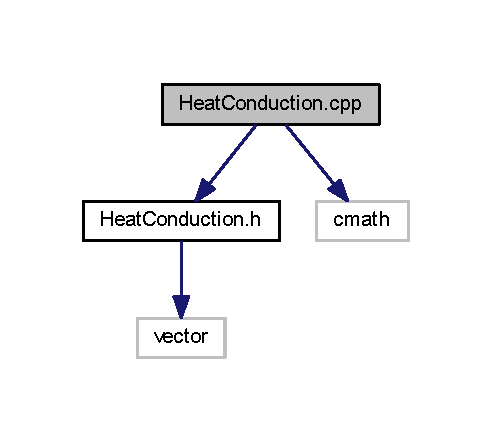
\includegraphics[width=236pt]{_heat_conduction_8cpp__incl}
\end{center}
\end{figure}
\subsection*{Variables}
\begin{DoxyCompactItemize}
\item 
\mbox{\Hypertarget{_heat_conduction_8cpp_a43016d873124d39034edb8cd164794db}\label{_heat_conduction_8cpp_a43016d873124d39034edb8cd164794db}} 
const double \hyperlink{_heat_conduction_8cpp_a43016d873124d39034edb8cd164794db}{pi} = atan(1) $\ast$ 4
\begin{DoxyCompactList}\small\item\em define pi \end{DoxyCompactList}\end{DoxyCompactItemize}


\subsection{Detailed Description}
Different objects to resolve an Heat Conduction problem. 

\begin{DoxyAuthor}{Author}
M Le Clec\textquotesingle{}h 
\end{DoxyAuthor}
\begin{DoxyVersion}{Version}
1.\+0 
\end{DoxyVersion}
\begin{DoxyDate}{Date}
05 December 2017
\end{DoxyDate}
There are 4 schemes which can be use \+:
\begin{DoxyItemize}
\item The Du\+Fort-\/\+Frankel scheme
\item The \hyperlink{class_richardson}{Richardson} scheme
\item The \hyperlink{class_laasonen}{Laasonen} scheme
\item The Crank-\/\+Nicholson scheme It can also provide the analytical solution. 
\end{DoxyItemize}
\hypertarget{_heat_conduction_8h}{}\section{Heat\+Conduction.\+h File Reference}
\label{_heat_conduction_8h}\index{Heat\+Conduction.\+h@{Heat\+Conduction.\+h}}


Different objects to resolve an Heat Conduction problem.  


{\ttfamily \#include $<$vector$>$}\newline
Include dependency graph for Heat\+Conduction.\+h\+:\nopagebreak
\begin{figure}[H]
\begin{center}
\leavevmode
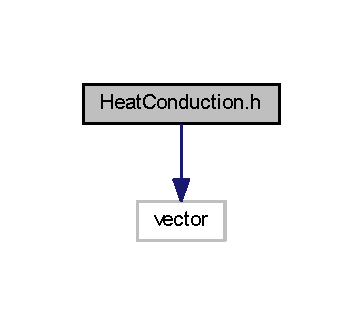
\includegraphics[width=174pt]{_heat_conduction_8h__incl}
\end{center}
\end{figure}
This graph shows which files directly or indirectly include this file\+:\nopagebreak
\begin{figure}[H]
\begin{center}
\leavevmode
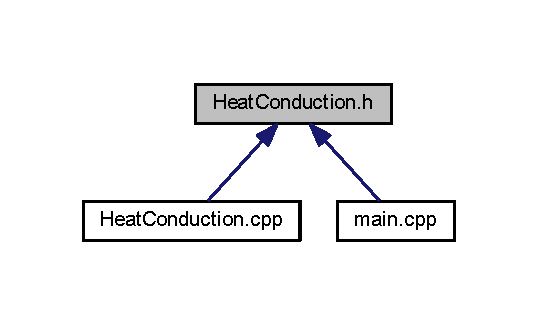
\includegraphics[width=258pt]{_heat_conduction_8h__dep__incl}
\end{center}
\end{figure}
\subsection*{Classes}
\begin{DoxyCompactItemize}
\item 
class \hyperlink{class_heat_conduction}{Heat\+Conduction}
\begin{DoxyCompactList}\small\item\em Base abstract Class which include all the parameters to solve the problem. \end{DoxyCompactList}\item 
class \hyperlink{class_analytical_solution}{Analytical\+Solution}
\begin{DoxyCompactList}\small\item\em Sub Class used to calculate the analytical solution. \end{DoxyCompactList}\item 
class \hyperlink{class_explicit_method}{Explicit\+Method}
\begin{DoxyCompactList}\small\item\em Sub Abstract Class used to calculate the Explicit scheme. \end{DoxyCompactList}\item 
class \hyperlink{class_implicit_method}{Implicit\+Method}
\begin{DoxyCompactList}\small\item\em Sub Abstract Class used to calculate the Implicit scheme. \end{DoxyCompactList}\item 
class \hyperlink{class_du_fort___frankel}{Du\+Fort\+\_\+\+Frankel}
\begin{DoxyCompactList}\small\item\em Sub sub Class used to calculate the \hyperlink{class_du_fort___frankel}{Du\+Fort\+\_\+\+Frankel} scheme. \end{DoxyCompactList}\item 
class \hyperlink{class_richardson}{Richardson}
\begin{DoxyCompactList}\small\item\em Sub sub Class used to calculate the \hyperlink{class_richardson}{Richardson} scheme. \end{DoxyCompactList}\item 
class \hyperlink{class_laasonen}{Laasonen}
\begin{DoxyCompactList}\small\item\em Sub sub Class used to calculate the \hyperlink{class_laasonen}{Laasonen} scheme. \end{DoxyCompactList}\item 
class \hyperlink{class_crank_nicholson}{Crank\+Nicholson}
\begin{DoxyCompactList}\small\item\em Sub sub Class used to calculate the Crank-\/\+Nicholson scheme. \end{DoxyCompactList}\end{DoxyCompactItemize}


\subsection{Detailed Description}
Different objects to resolve an Heat Conduction problem. 

\begin{DoxyAuthor}{Author}
M Le Clec\textquotesingle{}h 
\end{DoxyAuthor}
\begin{DoxyVersion}{Version}
1.\+0 
\end{DoxyVersion}
\begin{DoxyDate}{Date}
05 December 2017
\end{DoxyDate}
There are 4 schemes which can be use \+:
\begin{DoxyItemize}
\item The Du\+Fort-\/\+Frankel scheme
\item The \hyperlink{class_richardson}{Richardson} scheme
\item The \hyperlink{class_laasonen}{Laasonen} scheme
\item The Crank-\/\+Nicholson scheme It can also provide the analytical solution. 
\end{DoxyItemize}
\section{Norms.\+cpp File Reference}
\label{_norms_8cpp}\index{Norms.\+cpp@{Norms.\+cpp}}


Functions to calculates norms.  


{\ttfamily \#include \char`\"{}Norms.\+h\char`\"{}}\newline
\subsection*{Functions}
\begin{DoxyCompactItemize}
\item 
double \textbf{ norm\+\_\+one} (std\+::vector$<$ double $>$ solution)
\begin{DoxyCompactList}\small\item\em Function to calculate the first norm. \end{DoxyCompactList}\item 
double \textbf{ norm\+\_\+two} (std\+::vector$<$ double $>$ solution)
\begin{DoxyCompactList}\small\item\em Function to calculate the Euclidean norm. \end{DoxyCompactList}\item 
double \textbf{ norm\+\_\+uniform} (std\+::vector$<$ double $>$ solution)
\begin{DoxyCompactList}\small\item\em Function to calculate the Infinite norm. \end{DoxyCompactList}\end{DoxyCompactItemize}


\subsection{Detailed Description}
Functions to calculates norms. 

\begin{DoxyAuthor}{Author}
M Le Clec\textquotesingle{}h 
\end{DoxyAuthor}
\begin{DoxyVersion}{Version}
1.\+0 
\end{DoxyVersion}
\begin{DoxyDate}{Date}
05 December 2017
\end{DoxyDate}
There are 3 norms which can be calculated \+:
\begin{DoxyItemize}
\item The norm one
\item The norm two
\item The uniform norm 
\end{DoxyItemize}

\subsection{Function Documentation}
\mbox{\label{_norms_8cpp_a8a5dd7ae3578ecdb533ae37b7dd00086}} 
\index{Norms.\+cpp@{Norms.\+cpp}!norm\+\_\+one@{norm\+\_\+one}}
\index{norm\+\_\+one@{norm\+\_\+one}!Norms.\+cpp@{Norms.\+cpp}}
\subsubsection{norm\+\_\+one()}
{\footnotesize\ttfamily norm\+\_\+one (\begin{DoxyParamCaption}\item[{std\+::vector$<$ double $>$}]{solution }\end{DoxyParamCaption})}



Function to calculate the first norm. 


\begin{DoxyParams}{Parameters}
{\em solution} & Vector object on which we need to calculate the norm one. \\
\hline
\end{DoxyParams}
\begin{DoxyReturn}{Returns}
sum The result of the calculation. 
\end{DoxyReturn}


Definition at line 23 of file Norms.\+cpp.

\mbox{\label{_norms_8cpp_acde0d182617c91cb757a10b1bb2281f1}} 
\index{Norms.\+cpp@{Norms.\+cpp}!norm\+\_\+two@{norm\+\_\+two}}
\index{norm\+\_\+two@{norm\+\_\+two}!Norms.\+cpp@{Norms.\+cpp}}
\subsubsection{norm\+\_\+two()}
{\footnotesize\ttfamily norm\+\_\+two (\begin{DoxyParamCaption}\item[{std\+::vector$<$ double $>$}]{solution }\end{DoxyParamCaption})}



Function to calculate the Euclidean norm. 


\begin{DoxyParams}{Parameters}
{\em solution} & Vector object on which we need to calculate the second one. \\
\hline
\end{DoxyParams}
\begin{DoxyReturn}{Returns}
sum The result of the calculation. 
\end{DoxyReturn}


Definition at line 38 of file Norms.\+cpp.

\mbox{\label{_norms_8cpp_a87427a1c301886f335fd8485e638f9e2}} 
\index{Norms.\+cpp@{Norms.\+cpp}!norm\+\_\+uniform@{norm\+\_\+uniform}}
\index{norm\+\_\+uniform@{norm\+\_\+uniform}!Norms.\+cpp@{Norms.\+cpp}}
\subsubsection{norm\+\_\+uniform()}
{\footnotesize\ttfamily norm\+\_\+uniform (\begin{DoxyParamCaption}\item[{std\+::vector$<$ double $>$}]{solution }\end{DoxyParamCaption})}



Function to calculate the Infinite norm. 


\begin{DoxyParams}{Parameters}
{\em solution} & Vector object on which we need to calculate the uniform one. \\
\hline
\end{DoxyParams}
\begin{DoxyReturn}{Returns}
sum The result of the calculation. 
\end{DoxyReturn}


Definition at line 53 of file Norms.\+cpp.


\section{Norms.\+h File Reference}
\label{_norms_8h}\index{Norms.\+h@{Norms.\+h}}


Functions to calculates norms.  


{\ttfamily \#include $<$vector$>$}\newline
\subsection*{Functions}
\begin{DoxyCompactItemize}
\item 
double \textbf{ norm\+\_\+one} (std\+::vector$<$ double $>$ solution)
\begin{DoxyCompactList}\small\item\em Function to calculate the first norm. \end{DoxyCompactList}\item 
double \textbf{ norm\+\_\+two} (std\+::vector$<$ double $>$ solution)
\begin{DoxyCompactList}\small\item\em Function to calculate the Euclidean norm. \end{DoxyCompactList}\item 
double \textbf{ norm\+\_\+uniform} (std\+::vector$<$ double $>$ solution)
\begin{DoxyCompactList}\small\item\em Function to calculate the Infinite norm. \end{DoxyCompactList}\end{DoxyCompactItemize}


\subsection{Detailed Description}
Functions to calculates norms. 

\begin{DoxyAuthor}{Author}
M Le Clec\textquotesingle{}h 
\end{DoxyAuthor}
\begin{DoxyVersion}{Version}
1.\+0 
\end{DoxyVersion}
\begin{DoxyDate}{Date}
05 December 2017
\end{DoxyDate}
There are 3 norms which can be calculated \+:
\begin{DoxyItemize}
\item The norm one
\item The norm two
\item The uniform norm 
\end{DoxyItemize}

\subsection{Function Documentation}
\mbox{\label{_norms_8h_a4eb114881aa581e7043bd66e04ba27d0}} 
\index{Norms.\+h@{Norms.\+h}!norm\+\_\+one@{norm\+\_\+one}}
\index{norm\+\_\+one@{norm\+\_\+one}!Norms.\+h@{Norms.\+h}}
\subsubsection{norm\+\_\+one()}
{\footnotesize\ttfamily double norm\+\_\+one (\begin{DoxyParamCaption}\item[{std\+::vector$<$ double $>$}]{solution }\end{DoxyParamCaption})}



Function to calculate the first norm. 


\begin{DoxyParams}{Parameters}
{\em solution} & Vector object on which we need to calculate the norm one. \\
\hline
\end{DoxyParams}
\begin{DoxyReturn}{Returns}
sum The result of the calculation. 
\end{DoxyReturn}


Definition at line 23 of file Norms.\+cpp.

\mbox{\label{_norms_8h_a640d4f250d9b19707f3beef13f540f20}} 
\index{Norms.\+h@{Norms.\+h}!norm\+\_\+two@{norm\+\_\+two}}
\index{norm\+\_\+two@{norm\+\_\+two}!Norms.\+h@{Norms.\+h}}
\subsubsection{norm\+\_\+two()}
{\footnotesize\ttfamily double norm\+\_\+two (\begin{DoxyParamCaption}\item[{std\+::vector$<$ double $>$}]{solution }\end{DoxyParamCaption})}



Function to calculate the Euclidean norm. 


\begin{DoxyParams}{Parameters}
{\em solution} & Vector object on which we need to calculate the second one. \\
\hline
\end{DoxyParams}
\begin{DoxyReturn}{Returns}
sum The result of the calculation. 
\end{DoxyReturn}


Definition at line 38 of file Norms.\+cpp.

\mbox{\label{_norms_8h_a499e336aa7c1b95977115ce04115593c}} 
\index{Norms.\+h@{Norms.\+h}!norm\+\_\+uniform@{norm\+\_\+uniform}}
\index{norm\+\_\+uniform@{norm\+\_\+uniform}!Norms.\+h@{Norms.\+h}}
\subsubsection{norm\+\_\+uniform()}
{\footnotesize\ttfamily double norm\+\_\+uniform (\begin{DoxyParamCaption}\item[{std\+::vector$<$ double $>$}]{solution }\end{DoxyParamCaption})}



Function to calculate the Infinite norm. 


\begin{DoxyParams}{Parameters}
{\em solution} & Vector object on which we need to calculate the uniform one. \\
\hline
\end{DoxyParams}
\begin{DoxyReturn}{Returns}
sum The result of the calculation. 
\end{DoxyReturn}


Definition at line 53 of file Norms.\+cpp.


%--- End generated contents ---

% Index
\backmatter
\newpage
\phantomsection
\clearemptydoublepage
\addcontentsline{toc}{chapter}{Index}
\printindex

\end{document}
